\section{Conclusion and Learnings} \label{section:luckypatcher-learnings}
The summary of the \gls{lvl} patterns and their use in the patching modes can be seen in table~\ref{table:patterns}.
Amazon and Samsung are always successful since not the developer implementation is attacked but the library itself, which is always the same.
\newline
When patching Amazon, Samsung and the \gls{lvl} with the auto and inversed auto mode, the patches are applied determined to the important parts of the application.
They are effective as long as the library is not modified by the developer.
In contrast to the determined patching of the automatic modes, the extreme mode tries to apply patterns to files in other locations as well as to more complex methods.
This might cause instability, as seen in pattern N6, since it alters the syntax of the dex file.
\newline
\newline
Table~\ref{table:functionality} gives an overview of patched applications.
\gls{luckypatcherg} does not guarantee to be successful with one or more patching modes.
\newline
The first example is \textit{LicenseTest}.
While circumventing the license verification with the auto mode alone and combined with the extreme mode is possible, it does not work with the other modes.
One reason is due to the inversed auto mode tailored to the opposed configuration of the \textit{allowAccess()} method implemented.
Another reason is that the extreme mode is an addition to counter modified license verification implementations.
\newline
The second example is \textit{Runtastic Pro}.
This implementation is altered in a bad way which makes it vulnerable to all patching modes.
In the pirated and unmodified application, the user is told that the application is under maintenance.
When the patches are applied, the user can login as if the application was bought in the store.
\newline
The third example is \textit{Teamspeak 3}.
Their interpretation for the license verification is able to withstand all attacks.
\newline
\begin{table}
\centering
\begin{tabular}{llll}
                                             & \multicolumn{3}{c}{Application}             \\
\multicolumn{1}{c|}{Modus}                   & LicenseTest & Runtastic Pro & Teamspeak 3 \\ \hline
\multicolumn{1}{l|}{Purchased}               & yes           & yes           & yes         \\
\multicolumn{1}{l|}{Pirated}                 & no            & no            & no          \\
\multicolumn{1}{l|}{Auto}                    & yes           & yes           & no          \\
\multicolumn{1}{l|}{Auto (Inversed)}         & no            & yes           & no          \\
\multicolumn{1}{l|}{Extreme}                 & no            & yes           & no          \\
\multicolumn{1}{l|}{Auto+Extreme}            & yes           & yes           & no          \\
\multicolumn{1}{l|}{Auto (Inversed)+Extreme} & no            & yes           & no
\end{tabular}
\caption{Functionality for the test apps before and after patching}
\label{table:functionality}
\end{table}
\gls{luckypatcherg} is carrying out the attack by modifying the logic of the license verification libraries.
The circumvention of the verification process is achieved by apply only minor changes.
Single opcodes are changed to alter checks.
The resulting code evaluates a constant with desired outcome instead of the result of the initial method.
This way bad response codes can be ignored while the outcome is enforced.
It is very difficult to avoid this kind of attack since the license verification process is dependent on the binary \textit{yes/no} evaluation.
An abstraction of the unary verification mechanism is presented in figure~\ref{fig:verificationNow}.
\newline
\begin{figure}[h]
    \centering
    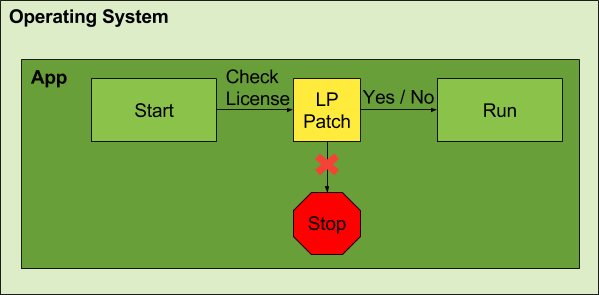
\includegraphics[width=0.8\textwidth]{data/verificationNowAttack.png}
    \caption{Abstraction of the current attack on the license verification mechanism}
    \label{fig:verificationNowAttack}
\end{figure}
The changes are applied by extracting, modifying and repacking the \textit{class.dex} similar to the build process of subsection~\ref{subsection:foundation-android-package}.
The modification of the file entails that its checksum and signature have to be recalculated.
Since Android can detect tampering of the \gls{apk}, the digest of the file in the \textit{META-INF} folder and its manifest files has to be adjusted as well \cite{androidSigning}.
\gls{luckypatcherg} does not have the developer's private key to sign the files accordingly.
This causes problems when certificate is checked for its origin but since Android allows self-signed certificates it does not matter \cite{codeSigning}.
Android just compares the certificates in case an application is updated with a \gls{apk} containing the same package name or when trust relationships between applications are about to be established. \cite{androidSigning}
The only limitation is the installation of the modified \gls{apk} is only possible when the original application is removed and future updates are not possible as long as the new \gls{apk} contains the same certificate.
\newline
The creation of the modified \gls{apk} does not require \textit{root} and the cracked \gls{apk} can be distributed without limitations.
This makes piracy easy for users and is a huge threat to developers.
